\documentclass[10pt, french]{article}

%% -----------------------------
%% Préambule
%% -----------------------------
% !TEX encoding = UTF-8 Unicode
% LaTeX Preamble for all cheatsheets
% Author : Gabriel Crépeault-Cauchon

% HOW-TO : copy-paste this file in the same directory as your .tex file, and add in your preamble the next command right after you have specified your documentclass : 
% \input{preamble-cheatsht.tex}
% ---------------------------------------------
% ---------------------------------------------

% Extra note : this preamble creates document that are meant to be used inside the multicols environment. See the documentation on internet for further information.

%% -----------------------------
%% Encoding packages
%% -----------------------------
\usepackage[utf8]{inputenc}
\usepackage[T1]{fontenc}
\usepackage{babel}
\usepackage{lmodern}
\usepackage[colorinlistoftodos]{todonotes}
%% -----------------------------
%% Variable definition
%% -----------------------------
\def\auteur{\href{https://github.com/ressources-act/Guide_de_survie_en_actuariat/blob/master/02_Cheatsheets/contributeurs/contributeurs-cheatshts.pdf}{\faGithub \ Liste des contributeurs}}
\def\BackgroundColor{white}
\usepackage{xargs} % for more logical new function creation

%% -----------------------------
%% Margin and layout
%% -----------------------------
% Determine the margin for cheatsheet
\usepackage[landscape, hmargin=1cm, vmargin=1.7cm]{geometry}
\usepackage{multicol}

% Remove automatic indentation after section/subsection title.
\setlength{\parindent}{0cm}

% Save space in cheatsheet by removing space between align environment and normal text.
\usepackage{etoolbox}
\newcommand{\zerodisplayskips}{%
  \setlength{\abovedisplayskip}{0pt}%
  \setlength{\belowdisplayskip}{0pt}%
  \setlength{\abovedisplayshortskip}{0pt}%
  \setlength{\belowdisplayshortskip}{0pt}}
\appto{\normalsize}{\zerodisplayskips}
\appto{\small}{\zerodisplayskips}
\appto{\footnotesize}{\zerodisplayskips}

%% -----------------------------
%% URL and links
%% -----------------------------
\usepackage{hyperref}
\hypersetup{colorlinks = true, urlcolor = gray!70!white, linkcolor = black}

%% -----------------------------
%% Document policy (uncomment only one)
%% -----------------------------
%	\usepackage{concrete}
	\usepackage{mathpazo}
%	\usepackage{frcursive} %% permet d'écrire en lettres attachées
%	\usepackage{aeguill}
%	\usepackage{mathptmx}
%	\usepackage{fourier} 

%% -----------------------------
%% Math configuration
%% -----------------------------
\usepackage[fleqn]{amsmath}
\usepackage{amsthm,amssymb,latexsym,amsfonts}
\usepackage{gensymb}
\usepackage{empheq}
\usepackage{numprint}
\usepackage{dsfont} % Pour avoir le symbole du domaine Z
%\usepackage{bigints} % pour des gros intégrales
% Mathematics shortcuts
\usepackage{scalerel,stackengine,amsmath}
\newcommand\equalhat{\mathrel{\stackon[1.5pt]{=}{\stretchto{%
    \scalerel*[\widthof{=}]{\wedge}{\rule{1ex}{3ex}}}{0.5ex}}}}
\newcommand{\reels}{\mathbb{R}}
\newcommand{\entiers}{\mathbb{Z}}
\newcommand{\naturels}{\mathbb{N}}
\newcommand{\eval}{\biggr \rvert}
\usepackage{cancel}
\newcommand{\derivee}[1]{\frac{\partial}{\partial #1}}
\newcommand{\prob}[1]{\Pr \left( #1 \right)}
\newcommand{\esp}[1]{\mathrm{E} \left[ #1 \right]} % espérance
\newcommand{\variance}[1]{\mathrm{Var} \left( #1   \right)}
\newcommand{\covar}[1]{\mathrm{Cov} \left( #1   \right)}
\newcommand{\laplace}{\mathcal{L}}
\newcommand{\deriv}[3][]{\frac{\partial^{#1}#3}{\partial #2^{#1}}}
\newcommand{\e}[1]{\mathrm{e}^{#1}}
\newcommand{\te}[1]{\text{exp}\left\{#1\right\}}
\DeclareMathSymbol{\shortminus}{\mathbin}{AMSa}{"39}
%%	Example usage:	\sumz{n}{i = 1} <=> \overset{n}{\underset{i = 1}{\sum}}
\newcommand{\sumz}[2]{\overset{#1}{\underset{#2}{\sum}}}
%%	Example usage:	\limz{h}{0} <=> \underset{h \rightarrow 0}{\lim}
\newcommand{\limz}[2]{\underset{#1 \rightarrow #2}{\lim}}
%%	Example usage:	\LVx{h}	<=>	\actsymb[h]{L}{}[]
%%					\LVx[n]{h}	<=>	\actsymb[h]{L}{}[n]
\newcommand{\LVx}[2][]{\actsymb[#2]{L}{}[#1]}
\DeclareMathOperator*{\argmax}{arg\,max}
\DeclareMathOperator*{\argmin}{arg\,min}
%%%	\icbox{<frame color>}{<background color>}{<text>}
\newcommandx{\icbox}[3][1 = bleudefrance, 2 = beaublue]{\fcolorbox{#1}{#2}{#3}}
%%	other good color combo is azure(colorwheel) arsenic
\usepackage{longfbox}
%	voir cette page, paquetage avec CSS https://ctan.math.illinois.edu/macros/latex/contrib/longfbox/longfbox.html
\newfboxstyle{rappel}{
	background-color = tealblue!20!white, 
	border-style = outset,
	breakable = true,
%	
	border-color = tealblue,
	border-radius = 1ex, 
%
	padding-bottom = 0.2ex,
	padding-top = 0.2ex,
	padding-left = 0.4ex,
	padding-right = 0.4ex,
%	
	border-top-width = 0.3ex,
	border-bottom-width = 0.3ex,
%
	border-left-width = 1ex, 
	border-bottom-left-radius = 0.2ex,
%	
	border-right-width = 1ex, 
	border-top-right-radius = 0.2ex,
%	
}
\newfboxstyle{formula}{ 
	background-color = beaublue, 
	border-color = bleudefrance
}
\newfboxstyle{imphl}{ 
	padding = 0pt,
	margin = 0pt,
	baseline-skip = false,
	background-color = palechestnut!60!white, 
	border-color = white
}
\newfboxstyle{conditions}{ 
	background-color = palechestnut, 
	border-color = red
}
\newcommandx{\rcbox}[3][1 = bleudefrance, 2 = beaublue]{\lfbox[border-radius = 0.5ex, background-color = #2, border-color = #1]{#3}}

% To indicate equation number on a specific line in align environment
\newcommand\numberthis{\addtocounter{equation}{1}\tag{\theequation}}

%
% Actuarial notation packages
%
\usepackage{actuarialsymbol}
\usepackage{actuarialangle}

%
% Matrix notation for math symbols (\bm{•})
%
\usepackage{bm}
% Matrix notation variable (bold style)
\newcommand{\matr}[1]{\mathbf{#1}}



%% -----------------------------
%% tcolorbox configuration
%% -----------------------------
\usepackage[most]{tcolorbox}
\tcbuselibrary{xparse}
\tcbuselibrary{breakable}

%%
%% Coloured box "definition" for definitions
%%
\DeclareTColorBox{definition}{ o }				% #1 parameter
{
	colframe=black,colback=white, % color of the box
	breakable, 
	pad at break* = 0mm, 						% to split the box
	title = {#1},
	after title = {\large \hfill \faBook},
}
%%
%% Coloured box "definition2" for definitions
%%
\DeclareTColorBox{definitionNOHFILL}{ o }				% #1 parameter
{
	colframe=blue!60!green,colback=blue!5!white, % color of the box
	pad at break* = 0mm, 						% to split the box
	title = {#1},
	before title = {\faBook \quad },
	breakable
}
%%
%% Coloured box "definition2" for definitions
%%
\DeclareTColorBox{definitionNOHFILLsub}{ o }				% #1 parameter
{
	colframe=blue!40!green,colback=blue!5!white, % color of the box
	pad at break* = 0mm, 						% to split the box
	title = {#1},
	before title = {\faNavicon \quad }, %faBars  faGetPocket
	breakable
}
%%
%% Coloured box "definition3" for propriétés
%%
\DeclareTColorBox{definitionNOHFILLprop}{ o }				% #1 parameter
{
	colframe=amber(sae/ece),colback=amber(sae/ece)!5!white, % color of the box
	pad at break* = 0mm, 						% to split the box
	title = {#1},
	before title = {\faGetPocket \quad }, %faBars  faGetPocket
	breakable
}
%%
%% Coloured box "definition3" for propriétés
%%
\DeclareTColorBox{definitionNOHFILLpropos}{ o }				% #1 parameter
{
	colframe=carmine,colback=carmine!5!white, % color of the box
	pad at break* = 0mm, 						% to split the box
	title = {#1},
	before title = {\faColumns \quad }, %\faEllipsisH  faColumns
	breakable
}


%%
%% Coloured box "algo" for algorithms
%%
\newtcolorbox{algo}[ 1 ]
{
	colback = blue!5!white,
	colframe = blue!75!black,
	title=#1,
	fonttitle = \bfseries,
	breakable
}
%%
%% Coloured box "conceptgen" for points adding to a concept's deifintion
%%
\newtcolorbox{conceptgen}[ 1 ]
{
	breakable,
	colback = beaublue,
	colframe = airforceblue,
	title=#1,
	fonttitle = \bfseries
}
%%
%% Coloured box "rappel" pour rappel de formules
%%
\DeclareTColorBox{conceptgen_enhanced}{ o }
{
	enhanced,
	title = #1,
	colback=beaublue, % color of the box
%	colframe=blue(pigment),
%	colframe=arsenic,	
	colbacktitle=airforceblue,
	fonttitle = \bfseries,
	breakable,
	boxed title style={size=small,colframe=arsenic} ,
	attach boxed title to top center = {yshift=-3mm,yshifttext=-1mm},
}
%%
%% Coloured box "probch1" pour formules relatives au 1er chapitre de prob
%%
\newtcolorbox{probch1}[ 1 ]
{
	colback = ao(english)!40!white,
	colframe = forestgreen(traditional),
	fonttitle = \bfseries,	
	breakable,
	title=#1
}
%%
%% Coloured box "probch2" pour formules relatives au 2e chapitre de prob
%%
\newtcolorbox{probch2}[ 1 ]
{
	colback = orange!50!white,
	colframe = burntorange,
	fonttitle = \bfseries,	
	breakable,
	title=#1
}
%%
%% Coloured box "axioms" pour formules relatives à la dernière partie du chapitre 2 de prob
%%
\newtcolorbox{axioms}[ 1 ]
{
	colback = blue!10!white,
	colframe = blue!70!white,
	fonttitle = \bfseries,	
	breakable,
	title=#1
}
%%
%% Coloured box "probch3" pour formules relatives au 3ème chapitre de prob
%%
\newtcolorbox{probch3}[ 1 ]
{
	colback = ruddypink,
	colframe = burgundy,
	fonttitle = \bfseries,	
	breakable,
	title=#1
}
%%
%% Coloured box "formula" for formulas
%%
\newtcolorbox{formula}[ 1 ]
{
	colback = green!5!white,
	colframe = green!70!black,
	breakable,
	fonttitle = \bfseries,
	title=#1
}
%%
%% Coloured box "formula" for formulas
%%
\DeclareTColorBox{algo2}{ o }
{
	enhanced,
	title = #1,
	colback=blue!5!white,	
	colbacktitle=blue!75!black,
	fonttitle = \bfseries,
	breakable,
	boxed title style={size=small,colframe=arsenic} ,
	attach boxed title to top center = {yshift=-3mm,yshifttext=-1mm},
}
%%
%% Coloured box "examplebox" for formulas
%%
\newtcolorbox{examplebox}[ 1 ]
{
	colback = beaublue,
	colframe = amethyst,
	breakable,
	fonttitle = \bfseries,title=#1
}
%%
%% Coloured box "rappel" pour rappel de formules
%%
\newtcolorbox{rappel}[ 1 ]
{
	colback = ashgrey,
	colframe = arsenic,
	breakable,
	fonttitle = \bfseries,title=#1
}
%%
%% Coloured box "rappel" pour rappel de formules
%%
\DeclareTColorBox{rappel_enhanced}{ o }
{
	enhanced,
	title = #1,
	colback=ashgrey, % color of the box
%	colframe=blue(pigment),
%	colframe=arsenic,	
	colbacktitle=arsenic,
	fonttitle = \bfseries,
	breakable,
	boxed title style={size=small,colframe=arsenic} ,
	attach boxed title to top center = {yshift=-3mm,yshifttext=-1mm},
}
%%
%% Coloured box "notation" for notation and terminology
%%
\DeclareTColorBox{distributions}{ o }			% #1 parameter
{
	enhanced,
	title = #1,
	colback=gray(x11gray), % color of the box
%	colframe=blue(pigment),
	colframe=arsenic,	
	colbacktitle=aurometalsaurus,
	fonttitle = \bfseries,
	boxed title style={size=small,colframe=arsenic} ,
	attach boxed title to top center = {yshift=-3mm,yshifttext=-1mm},
	breakable
%	left=0pt,
%  	right=0pt,
%    box align=center,
%    ams align*
%  	top=-10pt
}
\newtcolorbox{contrib}[ 1 ]
{
	colback = babyblueeyes,
	colframe = airforceblue,
	fonttitle = \bfseries,
	title = {#1},
	valign = center
}

%% -----------------------------
%% Graphics and pictures
%% -----------------------------
\usepackage{graphicx}
\usepackage{pict2e}
\usepackage{tikz}

%% -----------------------------
%% insert pdf pages into document
%% -----------------------------
\usepackage{pdfpages}

%% -----------------------------
%% Color configuration
%% -----------------------------
\usepackage{color, soulutf8, colortbl}


%
%	Colour definitions
%
\definecolor{armygreen}{rgb}{0.29, 0.33, 0.13}	%	army
\definecolor{asparagus}{rgb}{0.53, 0.66, 0.42}	% pastel green militariesque
\definecolor{britishracinggreen}{rgb}{0.0, 0.26, 0.15}
\definecolor{calpolypomonagreen}{rgb}{0.12, 0.3, 0.17}
\definecolor{darkgreen}{rgb}{0.0, 0.2, 0.13}
\definecolor{lightgreen}{rgb}{0.2, 0.95, 0.2}

\definecolor{antiquebrass}{rgb}{0.8, 0.58, 0.46}	% brown-ish light cardboard color

\definecolor{blue(munsell)}{rgb}{0.0, 0.5, 0.69}
\definecolor{blue(matcha)}{rgb}{0.596, 0.819, 1.00}
\definecolor{blue(munsell)-light}{rgb}{0.5, 0.8, 0.9}
\definecolor{bleudefrance}{rgb}{0.19, 0.55, 0.91}
\definecolor{blizzardblue}{rgb}{0.67, 0.9, 0.93}	%	mr.freeze light baby blue 
\definecolor{bondiblue}{rgb}{0.0, 0.58, 0.71}	%	darker cyan type inidgo blue
\definecolor{blue(pigment)}{rgb}{0.2, 0.2, 0.6}
\definecolor{bluebell}{rgb}{0.64, 0.64, 0.82}
\definecolor{airforceblue}{rgb}{0.36, 0.54, 0.66}
\definecolor{beaublue}{rgb}{0.74, 0.83, 0.9}    % almost white
\definecolor{blue_rectangle}{RGB}{83, 84, 244}		% ACT-2004
\definecolor{cobalt}{rgb}{0.0, 0.28, 0.67}	% nice light blue-ish
\definecolor{ballblue}{rgb}{0.13, 0.67, 0.8}	%	almost green ish blue ish
\definecolor{babyblueeyes}{rgb}{0.63, 0.79, 0.95}

\definecolor{indigo(web)}{rgb}{0.29, 0.0, 0.51}	% purple-ish
\definecolor{antiquefuchsia}{rgb}{0.57, 0.36, 0.51}	%	pastel matte (darkerish) purple ish
\definecolor{darkpastelpurple}{rgb}{0.59, 0.44, 0.84}	%	pretty purple
\definecolor{gray(x11gray)}{rgb}{0.75, 0.75, 0.75}
\definecolor{aurometalsaurus}{rgb}{0.43, 0.5, 0.5}
\definecolor{bulgarianrose}{rgb}{0.28, 0.02, 0.03}	%	dark maroon type 
\definecolor{pastelred}{rgb}{1.0, 0.41, 0.38}		%	light red pinktinybit ish
\definecolor{lightmauve}{rgb}{0.86, 0.82, 1.0}
\definecolor{eggshell}{rgb}{0.94, 0.92, 0.84}
\definecolor{azure(colorwheel)}{rgb}{0.0, 0.5, 1.0}
\definecolor{darkgreen}{rgb}{0.0, 0.2, 0.13}			
\definecolor{ao(english)}{rgb}{0.0, 0.5, 0.0}		% prertty apple dark pastel (light) green
\definecolor{green_rectangle}{RGB}{131, 176, 84}		% ACT-2004
\definecolor{red_rectangle}{RGB}{241,112,113}		% ACT-2004
\definecolor{amethyst}{rgb}{0.6, 0.4, 0.8}
\definecolor{amethyst-light}{rgb}{0.6, 0.4, 0.8}
\definecolor{ruddypink}{rgb}{0.88, 0.56, 0.59}

\definecolor{amber(sae/ece)}{rgb}{1.0, 0.49, 0.0} 	%	pretty orange ish
\definecolor{burntsienna}{rgb}{0.91, 0.45, 0.32}		%%	lighter pastel orange
\definecolor{burntorange}{rgb}{0.8, 0.33, 0.0}		%%	similar but deeper orange
\definecolor{orange-red}{rgb}{1.0, 0.27, 0.0}

\definecolor{tealblue}{rgb}{0.21, 0.46, 0.53}

\definecolor{battleshipgrey}{rgb}{0.52, 0.52, 0.51}  % lilght ish gray
\definecolor{ashgrey}{rgb}{0.7, 0.75, 0.71}			% dark grey-black-ish
\definecolor{arsenic}{rgb}{0.23, 0.27, 0.29}			% light green-beige-ish gray
\definecolor{gray(x11gray)}{rgb}{0.75, 0.75, 0.75}

\definecolor{carmine}{rgb}{0.59, 0.0, 0.09} 			% deep red
\definecolor{amaranth}{rgb}{0.9, 0.17, 0.31}
\definecolor{brickred}{rgb}{0.8, 0.25, 0.33}
\definecolor{chestnut}{rgb}{0.8, 0.36, 0.36}		% pink red ish light
\definecolor{palechestnut}{rgb}{0.87, 0.68, 0.69}
\definecolor{pastelred}{rgb}{1.0, 0.41, 0.38}
\definecolor{forestgreen(traditional)}{rgb}{0.0, 0.27, 0.13}
%
% Useful shortcuts for coloured text
%
\newcommand{\orange}{\textcolor{orange}}
\newcommand{\red}{\textcolor{red}}
\newcommand{\cyan}{\textcolor{cyan}}
\newcommand{\blue}{\textcolor{blue}}
\newcommand{\green}{\textcolor{green}}
\newcommand{\purple}{\textcolor{magenta}}
\newcommand{\yellow}{\textcolor{yellow}}

%% -----------------------------
%% Enumerate environment configuration
%% -----------------------------
%
% Custum enumerate & itemize Package
%
\usepackage{enumitem}
%
% French Setup for itemize function
%
\frenchbsetup{StandardItemLabels=true}
%
% Change default label for itemize
%
\renewcommand{\labelitemi}{\faAngleRight}


%% -----------------------------
%% Tabular column type configuration
%% -----------------------------
\newcolumntype{C}{>{$}c<{$}} % math-mode version of "l" column type
\newcolumntype{L}{>{$}l<{$}} % math-mode version of "l" column type
\newcolumntype{R}{>{$}r<{$}} % math-mode version of "l" column type
\newcolumntype{f}{>{\columncolor{green!20!white}}p{1cm}}
\newcolumntype{g}{>{\columncolor{green!40!white}}m{1.2cm}}
\newcolumntype{a}{>{\columncolor{red!20!white}$}p{2cm}<{$}}	% ACT-2005
% configuration to force a line break within a single cell
\usepackage{makecell}


%% -----------------------------
%% Fontawesome for special symbols
%% -----------------------------
\usepackage{fontawesome}

%% -----------------------------
%% Section Font customization
%% -----------------------------
\usepackage{sectsty}
\sectionfont{\color{\SectionColor}}
\subsectionfont{\color{\SubSectionColor}}
\subsubsectionfont{\color{\SubSubSectionColor}}

%% -----------------------------
%% Footer/Header Customization
%% -----------------------------
\usepackage{lastpage}
\usepackage{fancyhdr}
\pagestyle{fancy}

%
% Header
%
\fancyhead{} 	% Reset
\fancyhead[L]{Aide-mémoire pour~ \cours ~(\textbf{\sigle})}
\fancyhead[R]{\auteur}

%
% Footer
%
\fancyfoot{}		% Reset
\fancyfoot[R]{\thepage ~de~ \pageref{LastPage}}
\fancyfoot[L]{\href{https://github.com/ressources-act/Guide_de_survie_en_actuariat}{\faGithub \ ressources-act/Guide de survie en actuariat}}
%
% Page background color
%
\pagecolor{\BackgroundColor}




%% END OF PREAMBLE
% ---------------------------------------------
% ---------------------------------------------
%% -----------------------------
%% Variable definition
%% -----------------------------
\def\cours{Introduction à l'actuariat II}
\def\sigle{ACT-2001}
\def\SectionColor{burntorange}
\def\SubSectionColor{burntsienna}
\def\SubSubSectionColor{burntsienna}

%% Reduce margin space
\setlength{\abovedisplayskip}{-15pt}
\setlist{leftmargin=*}

\newcommand{\bettershortstack}[2][c]{%
  \begin{tabular}[b]{@{}#1@{}}#2\end{tabular}%
}
\usepackage{stackengine}
\newcommand\cumlaut[2][black]{\stackon[.33ex]{#2}{\textcolor{#1}{\kern-.04ex.\kern-.2ex.}}}
%% -----------------------------
%% Début du document
%% -----------------------------
\begin{document}

\begin{center}
	\textsc{\Large Contributeurs}\\[0.5cm] 
\end{center}
%\input{contributeurs/contrib-ACT2001}

\newpage

\raggedcolumns
\begin{multicols*}{2} 

\section{Notions de base à la modélisation en actuariat}
\begin{distributions}[Notation]
\begin{description}
	\item[$X$]	Variable aléatoire représentant les pertes pour une "\textit{entité}" pour un (ou plusieurs) "\textit{périls}".
		\begin{itemize}
		\item	Elle peut être continue, discrète ou mixte ;
		\item	"\textit{Entité}" peut être un individu (ou groupe de), commerce, compagnie, etc. ;
		\item	"\textit{Périls}" peut être une incendie, du vandalisme, une maladie, du risque opérationnel, etc. ;
		\item	On pose que \lfbox[conditions]{$\text{E}[X]	<	\infty$}.
		\end{itemize}
	\item[$\text{PP}(X)$]	La \textbf{prime pure} pour le risque $X$, \lfbox[formula]{$\text{PP}(X)	=	\text{E}[X]$}.
\end{description}
\end{distributions}


\subsection{Fonction quantile}
\lfbox[formula]{$F_{X}^{-1}(u)	=	\inf\{x \in \mathbb{R}; F_{X}(x)	\geq u\}$}, \lfbox[conditions]{$\forall u \in (0, 1)$}.\\


\begin{formula}{\hyperlink{proof:ftc-quantile}{Théorème de la fonction quantile}}
Soit :	
\begin{itemize}
	\item	la variable aléatoire $X$ avec fonction de répartition $F_{X}(x)$ et la fonction quantile $F_{X}^{-1}(u)$.
	\item	la variable aléatoire $U \sim Unif(0, 1)$.
	\item	$Y	=	F_{X}^{-1}(U)$.
\end{itemize}

Alors, \lfbox[formula]{$F_{Y}(x)	=	F_{F_{X}^{-1}(U)}(x)	=	F_{X}(x)$} \lfbox[conditions]{$\forall x \in \mathbb{R}$} et \lfbox[formula]{$X		=	F_{X}^{-1}(U)$}.

\tcbline

C'est-à-dire, on défini $Y$ comme la transformation de la variable aléatoire $U$ via la fonction quantile. Par conséquent, $Y$ se comporte comme $X$.
\end{formula}

\setcounter{subsection}{3}
\subsection{Espérance tronquée}
On pose que $X$ est une variable aléatoire tel que $\text{E}[X]	<	\infty$.
\begin{distributions}[Notation]
\begin{description}
	\item[]	$\text{E}[X \times \bm{1}_{\{X > d\}}]$	l'espérance tronquée à $d$.
		\begin{itemize}
		\item	C'est-à-dire, l'espérance des valeurs de la v.a. $X$ qui sont supérieur à $d$.
		\item	On peut définir l'espérance tronquée avec n'importe quelle indicatrice.
		\end{itemize}
\end{description}
\end{distributions}

\textbf{Rappel :}
\begin{align*}
	\bm{1}_{\{X	>	d\}}
	&=	\begin{cases}	
		1,	&	X	>	d	\\
		0,	&	X	\leq	d	
		\end{cases}
\end{align*}


\subsection{Fonction \textbf{stop-loss}}
On pose que $X$ est une variable aléatoire tel que $\text{E}[X]	<	\infty$.
\begin{distributions}[Notation]
\begin{description}
	\item[$\pi_{X}(d)$]	Fonction stop-loss de déductible $d$ tel que \lfbox[formula]{$\pi_{X}(d)	=	\text{E}[\max\{X	-	d;	0\}]$}, \lfbox[conditions]{$\forall d \in \mathbb{R}$}.
		\begin{itemize}
		\item	C'est-à-dire, l'espérance des montants de perte en excédant de la limite $d$,
		\end{itemize}
\end{description}
\end{distributions}

\textbf{Relation :}
\begin{align*}
	\pi_{X}(d)
	&\equiv	\text{E}[X	\times	\bm{1}_{\{X	>	d\}}]	-	d\bar{F}_{X}(d)
\end{align*}


\subsection{Fonction quantile et espérance(s)}
\lfbox[formula]{$\text{E}[X]	=	\text{E}[F_{X}^{-1}(U)]	=	\int_{0}^{1}F_{X}^{-1}(u)du$}.

\textbf{Relation :}
\begin{align*}
	\int_{k}^{1}F_{X}^{-1}(u)du
	&=	\pi_{x}\left(F_{X}^{-1}(\kappa)\right) + (1 - \kappa)F_{X}^{-1}(\kappa), \quad \forall \kappa \in (0, 1)	\\
	&=	\text{E}\Big[X	\times	\bm{1}_{\{X	>	F_{X}^{-1}(\kappa)\}}\Big]+ 
		F_{X}^{-1}(\kappa)\bigg( F_{X}\Big(F_{X}^{-1}(\kappa)\Big)	-	\kappa \bigg)
\end{align*}

\subsection{Mesures de risque}
\begin{itemize}
	\item	La \textbf{Value-at-Risk} correspond au $100\alpha^{\text{e}}$ pourcentile;
%	\item	Si $X$ représente les pertes, on s'intéresse à l'extrémité supérieure de la distribution des gains et \icbox{$TVaR_{\kappa}(X)	=	\esp{X | X > \kappa}	=	\frac{1}{1 - \kappa} \int_{VaR_{\kappa}}^{\infty} x f_{X}(x)dx$} ;
%	\item	Si $X$ représente les gains, on s'intéresse à l'extrémité inférieure de la distribution des gains et \icbox{$TVaR_{\kappa}(X)	=	\esp{X | X \leq \kappa}	=	\frac{1}{\kappa} \int_{-\infty}^{VaR_{\kappa}} x f_{X}(x)dx$}.
\end{itemize}

Également, on a la $TVaR$ que l'on peut écrire pour $\kappa \in (0, 1)$: 
\begin{align*}
	TVaR_{\kappa}(X)
	&=	\frac{1}{1 - \kappa}\int_{\kappa}^{1}	VaR_{u}(X)du	\\
	&=	\frac{1}{1 - \kappa}\pi_{X}\left(VaR_{\kappa}(X)\right) + VaR_{\kappa}(X)	\\
	&=	\frac{1}{1 - \kappa}\left[	\text{E}[X \times \bm{1}_{\{X	>	VaR_{\kappa}(X)\}}] + VaR_{\kappa}(X) \left(F_{X}\left(VaR_{\kappa}(X)\right)	-	\kappa\right)	\right]
\end{align*}

Pour une variable aléatoire $X$ continue, on simplifie :
\begin{align*}
	TVaR_{\kappa}(X)
	&=	\frac{1}{1 - \kappa}\left[	\text{E}\left[X \times \bm{1}_{\{X	>	VaR_{\kappa}(X)\}}\right] + \underbrace{VaR_{\kappa}(X) \left(F_{X}\left(VaR_{\kappa}(X)\right)	-	\kappa\right)}_{\shortstack{= 0}}	\right]	\\
	&=	\frac{1}{1 - \kappa}\left[	\text{E}\left[X \times \bm{1}_{\{X	>	VaR_{\kappa}(X)\}}\right]	\right]	\\
	&\equiv	\frac{\text{E}\left[X \times \bm{1}_{\{X	>	VaR_{\kappa}(X)\}}\right]}{\Pr(X	>	VaR_{\kappa}(X))}	\\
	&=	\esp{X | X	>	Var_{\kappa}(X)}
\end{align*}

\subsubsection{Propriétés désirables d'une mesure de risque}
\begin{definitionNOHFILLsub}[Homogénéité]
Soit une v.a. $X$ et un scalaire \icbox[red][palechestnut]{$c	>	0$}, la mesure de risque $\rho$ est dite homogène si \icbox{$\rho(cX)	=	c\rho(X)$}.
\end{definitionNOHFILLsub}

\begin{definitionNOHFILLsub}[Invariance à la translation]
Soit une v.a. $X$ et un scalaire \icbox[red][palechestnut]{$c	\in	\mathbb{R}$}, la mesure de risque $\rho$ satisfait la propriété d'invariance à la translation si \icbox{$\rho(X + c)	=	\rho(X) + c$}.	\\

Ajouter un montant positif à un risque ajoute un montant équivalent à la mesure de risque.
\end{definitionNOHFILLsub}

\begin{definitionNOHFILLsub}[Monotonicité]
Soit les v.a. $X_{1}$ et $X_{2}$ \icbox[red][palechestnut]{tel que $\Pr(X	\leq	X_{2})	=	1$}, la mesure de risque $\rho$ satisfait la propriété de monotonicité si \icbox{$\rho(X_{1})	\leq	\rho(X_{2})$} ou si \icbox[red][palechestnut]{$\forall	u	\in	(0, 1)$}, \icbox{$F_{X_{1}}^{-1}(u)	\leq	F_{X_{2}}^{-1}(u)$}.
\end{definitionNOHFILLsub}

\begin{definitionNOHFILLsub}[Sous-additivité]
Soit les v.a. $X_{1}$ et $X_{2}$, la mesure de risque $\rho$ satisfait la propriété de sous-additivité si \icbox{$\rho(X_{1}	+	X_{2})	\leq	\rho(X_{1})	+	\rho(X_{2})$}.
\end{definitionNOHFILLsub}

\begin{definitionNOHFILLsub}[Convexité]
Soit les v.a. $X_{1}$ et $X_{2}$, la mesure de risque $\rho$ satisfait la propriété de convexité si \icbox{$\rho(\alpha X_{1}	+	(1	-	\alpha)X_{2})	\leq	\alpha\rho(X_{1})	+	(1	-	\alpha)\rho(X_{2})$}.
\end{definitionNOHFILLsub}



\pagebreak
\section{Méthodes de simulation Monte-Carlo}
\begin{algo2}[Méthode inverse]
Pour $j	=	1, 2, \dots, m$, 
\begin{enumerate}
	\item	On produit une réalisation $U^{(j)}$ d'une loi $U(0, 1)$ à partir d'un GNPA (\texttt{runif} en \texttt{R}).
	\item	On simule une réalisation $X^{(j)}$ de $X$ où \lfbox[formula]{$X^{(j)}	=	F_{X}^{-1}(U^{(j)})$}.
\end{enumerate}
\end{algo2}

\begin{algo2}[Simulation d'une fonction d'un nombre fini de variables aléatoires]
Pour $j	=	1, 2, \dots, m$, 
\begin{enumerate}
	\item	On simule les réalisations $\left(X_{1}^{(j)}, X_{2}^{(j)}, \dots, X_{n}^{(j)}\right)$ de $\left(X_{1}, X_{2}, \dots, X_{n}\right)$.
	\item	On évalue $Z^{(j)}	=	\phi\left(X_{1}^{(j)}, X_{2}^{(j)}, \dots, X_{n}^{(j)}\right)$.
\end{enumerate}

Par exemple, on peut avoir $\phi\left(x_{1}, x_{2}, \dots, x_{n}\right)	=	\sumz{n}{i = 1}x_{i}$.
\end{algo2}

\begin{algo2}[Simulation d'une fonction de variables aléatoires définies par un mélange]
Pour $j	=	1, 2, \dots, m$, 
\begin{enumerate}
	\item	On simule une réalisation $\Theta^{(j)}$ de $\Theta$.
	\item	On produit une réalisation $X^{(j)}$ de $X$ avec la fonction quantile $F_{X | \Theta = \Theta^{(j)}}$ de la fonction de répartition conditionnelle de $(X | \Theta = \Theta^{(j)})$
\end{enumerate}
\end{algo2}

\subsection{Erreur et intervalle de confiance}
Soit une v.a. $X$ dont on produit $m$ réalisation $\left( X^{(1)}, X^{(2)}, \dots, X^{(m)} \right)$.\\
Soit la fonction intégrale de $X$, $g(X)$.\\
On obtient les approximations pour $\theta	=	\text{E}[g(X)]$ : 
\begin{align*}
	\theta	
	&=	\simeq	\hat{\theta}_{m}
	=	\frac{1}{m}\sumz{m}{j	=	1} g\left(X^{(j)}\right)	\\
	\text{Var}\left(\hat{\theta}_{m}\right)
	&=	\frac{1}{m}\text{Var}\left(g(X)\right)	\\
	\widehat{\text{Var}}\left(g(X)\right)
	&=	\frac{1}{m - 1} \sumz{m}{j	=	1} \left(g\left(X^{(j)}\right)	-	\hat{\theta}_{m}\right)^{2}
\end{align*}

De plus, 
\begin{align*}
	\theta \in \left[\hat{\theta}_{m} \pm \sqrt{\frac{\text{Var}\left(\hat{\theta}_{m}\right)}{m}} \Phi^{-1} \left(1 - \frac{\alpha}{2}\right)\right]
	\approx	\left[\hat{\theta}_{m} \pm \sqrt{\frac{\widehat{\text{Var}}\left(\hat{\theta}_{m}\right)}{m}} \Phi^{-1} \left(1 - \frac{\alpha}{2}\right)\right]
\end{align*}

Également, la fonction de répartition peut être approximée avec $m$ réalisations $\left( X^{(1)}, X^{(2)}, \dots, X^{(m)} \right)$ :
\begin{align*}
	F^{(m)}_{X}(x)
	&\simeq	\frac{1}{m} \sumz{m}{j	=	1} \bm{1}_{\{X^{(j)}	\leq	x\}}
\end{align*}

De plus, pour \lfbox[conditions]{$j_{0}	=	m\times k$} entier :
\begin{align*}
	TVaR_{\kappa}(X)
	&\simeq	\frac{1}{m - j_{0}} \left( \frac{1}{m} \sumz{m}{j	=	j_{0} + 1} X^{[j]} 
%	+ X^{[j_{0}]}\bigg(F^{(m)}\big(X^{[j_{0}]}\big) - \kappa \bigg) 
	\right)
\end{align*}

\pagebreak
\section{Mutualisation des risques}
\begin{distributions}[Terminologie]
\begin{description}
	\item[$S$]	Pertes totales 
\end{description}
\end{distributions}

\subsection{Méthode de Monte-Carlo}
\begin{algo2}[Étapes pour simuler]
\begin{enumerate}
	\item	Produire $M$ réalisations $U^{(1)}, \dots, U^{(m)}$ de $U$ ;
	\item	Approximer $\theta$ par $\hat{\theta}_{m}$ où :
		\begin{align*}
		\hat{\theta}_{m}
		&=	\frac{1}{m} \sumz{m}{j = 1} \phi\left( F_{X}^{-1}\left(U^{(j)}\right) \right)	\\
		&=	\frac{1}{m} \sumz{m}{j = 1} \phi\left( X^{(j)} \right)	\\
		\end{align*}
\end{enumerate}
Par la loi des grands nombres, $\hat{\theta}_{m}	\overset{P}{\rightarrow}	\theta$.
\end{algo2}


\subsection{Mesures de risque}


\begin{description}
	\item[Capital économique]	Allocation de surplus de la compagnie;
		\begin{align*}
		CE(S)	
		&=	\rho(S)	-	\esp{S}
		\end{align*}
	\item[Marge de risque]	associée à une prime $P(X)$;
		\begin{align*}
		MR(X)
		&=	\rho(X)	-	\esp{X}
		\end{align*}
\end{description}

$\rho$ introduit une marge de risque:
\begin{description}
	\item[positive]	lorsque \icbox{$\rho(X)	\geq		\esp{X}$} pour une v.a. $X$ avec \icbox[red][palechestnut]{$\esp{X} < \infty$};
	\item[justifiée]	lorsque \icbox{$\rho(X)	=	\rho(a)	=	a$} pour une v.a. $X$ avec \icbox[red][palechestnut]{$\Pr(X	=	a)	=	1, \alpha > 0$};
	\item[non-excessive]	lorsque \icbox{$\rho(X)	\leq		a_{\max}$} pour une v.a. $X$ \icbox[red][palechestnut]{s'il existe $a_{\max}	<	\infty$} \icbox[red][palechestnut]{tel que $\Pr(X	\leq		a_{\max})	=	1$};
\end{description}

\pagebreak
\section{Modèles de risques non-vie}
\begin{distributions}[Notation]
\begin{description}
	\item[$M$]	Variable aléatoire du nombre de sinistres pour un risque;
	\item[$B_{k}$]	Variable aléatoire du montant du $k^{\text{e}}$ sinistre.
\end{description}
\end{distributions}

\begin{definitionNOHFILL}[Modèle fréquence-sinistre]
On défini la v.a. $X$ comme étant les coûts (pertes) pour un risque tel que \icbox[red][palechestnut]{$\forall	M	>	0$}:
\begin{align*}
	X
	&=	\sum_{k	=	1}^{M} B_{k}
\end{align*}

\tcbline

\begin{align*}
	\esp{X}
	&=	\text{E}_{\text{M}}\left[\text{E}_{\text{B}}[X | M]\right]	\\
	&=	\text{E}[M]	\times	\text{E}[B]	\\
	\text{Var}(X)
	&=	\underbrace{\text{Var}_{\text{M}}(\text{E}_{\text{B}}[X | M])}_{\text{variabilité du \textit{nombre} de sinistres}}	+	\underbrace{\text{E}_{\text{M}}\left[\text{Var}_{\text{B}}(X | M)\right]}_{\text{variabilité du \textit{coût} par sinistre}}	\\
	&=	\text{E}[M]\text{Var}(B)	+	\text{E}^{2}[B]\text{Var}(M)	\\
\end{align*}

\tcbline

\begin{align*}
	F_{X}(x)
	&=	\Pr(M	=	0)	+	\sum_{k	=	1}^{\infty} \Pr(M	=	k)F_{B_{1}	+	\dots	+	B_{k}}(x)
\end{align*}

Par exemple, pour $B_{k}	\sim	\Gamma(\alpha,	\beta)$:
\begin{align*}
	F_{X}(x)
	&=	\Pr(M	=	0)	+	\sum_{k	=	1}^{\infty} \Pr(M	=	k)H(x;	\alpha k, \beta)
\end{align*}

\tcbline

\begin{align*}
	\mathcal{L}_{X}(t)
	&=	P_{M}\left(\mathcal{L}_{B}(t)\right), \quad	t > 0	\\
	\esp{X	\times	\bm{1}_{\{X	>	b\}}}
	&=	\sum_{k	=	1}^{\infty} \Pr(M	=	k)E\left[(B_{1}	+	\dots	+	B_{k})	\times	\bm{1}_{\{B_{1}	+	\dots	+	B_{k} > b\}}\right]
\end{align*}

Par exemple, pour $B_{k}	\sim	\Gamma(\alpha,	\beta)$:
\begin{align*}
	\esp{X	\times	\bm{1}_{\{X	>	b\}}}
	&=	\sum_{k	=	1}^{\infty} \Pr(M	=	k) \frac{k\alpha}{\beta} \overline{H}(b;	\alpha k + 1, \beta)
\end{align*}
\end{definitionNOHFILL}

\subsection{Simulation}
\begin{algo2}[Simulation de réalisations de $X$]
\begin{enumerate}
	\item	Simuler la réalisation $M^{(j)}$ de la v.a. $M$ ;
	\item	Si $M^{(j)}	=	0$, alors $X^{(j)}	=	0$ ;
	\item	Si $M^{(j)}	>	0$, alors :	
		\begin{enumerate}
		\item	Simuler $M^{(j)}$ réalisations de la v.a. (iid) $B$ pour obtenir $B^{(j)}_{1}, B^{(j)}_{2}, \dots, B^{(j)}_{M^{(j)}}$;
		\item	On pose $X^{(j)}	=	B^{(j)}_{1} + B^{(j)}_{2} + \dots + B^{(j)}_{M^{(j)}}$.
		\end{enumerate}
\end{enumerate}
\end{algo2}

\subsection{Heavy tailed and light tailed}
Si la distribution de la v.a. $B$ est sub-exponentielle alors :
\begin{align*}
	\overline{F}_{X}(x)
	&=	\sumz{\infty}{k	=	1}f_{M}(k) \overline{F}_{B_{1} + \dots + B_{k}}(x)
	\sim	\sumz{\infty}{k	=	1}f_{M}(k)k\overline{F}_{B}(x)
	=	\text{E}[M]\overline{F}_{B}(x)
\end{align*}


\newpage
\part{ACT-3000: Théorie du risque}
\setcounter{section}{9}
\section{Processus de Poisson}
\begin{distributions}[Notation]
\begin{description}
	\item[$T_{k}$]	Temps d'occurrence de l'événement $k	=	1, 2, \dots$.
		\begin{itemize}
		\item	Il s'ensuit que \lfbox[conditions]{$0	<	T_{1}	<	T_{2}	<	\dots$} ;
		\item	\lfbox[formula]{$T_{k}	\sim	Erlang(k; \lambda)$}.
		\end{itemize}
	\item[$W_{k}$]	Temps écoulé entre l'événement $k - 1$ et $k$.
		\begin{itemize}
		\item	Il s'ensuit que \lfbox[formula]{$W_{k}	=	T_{k} - T_{k - 1}$} ;
		\item	\lfbox[formula]{$W_{k}	\sim	W	\sim	Exp(\lambda)$}.
		\end{itemize}
\end{description}
\end{distributions}

\begin{definitionNOHFILL}[Processus de comptage]
Soit le processus de comptage \lfbox[formula]{$\underline{N}	=	\{N(t), t \geq 0\}$} sous les conditions suivantes :
\begin{enumerate}
	\item	$N(0)	=	0$ ;
	\item	$N(t)	\geq	0$ ;
	\item	$N(t)	\geq	N(s)$ si $t	>	s$ ;
	\item	$N(t) - N(s)$ correspond au nombre d'événements encourus durant l'intervalle $(s, t]$ où $t	>	s$ ;
\end{enumerate}

Au lieu de le définir en fonction d'une loi de Poisson, on peut définir \lfbox[formula]{$N(t)	=	\sup\{k \geq 1 : T_{k} \leq t\}$}, \lfbox[conditions]{$\forall t \geq 0$}. C'est-à-dire, le dernier événement à se produire à ou avant le temps $t$.

\tcbline

\begin{itemize}
	\item	Alias, processus de dénombrement.
\end{itemize}
\end{definitionNOHFILL}


\columnbreak
\subsection{Processus de Poisson homogène}
\begin{distributions}[Notation]
\begin{description}
	\item[$\lambda$]	Taux, ou intensité, du processus.
	\item[$\Lambda(t)$]	Intensité cumulée :
		\begin{align*}
		\Lambda(t)
		&=	\int_{0}^{t} \lambda ds
		=	\lambda t, \quad t > 0
		\end{align*}
\end{description}
\end{distributions}

\begin{definitionNOHFILLsub}[Processus de Poisson]
$\underline{N}	=	\{N(t), t \geq 0\}$ est un \textbf{processus de Poisson} sous les conditions suivantes :
\begin{enumerate}
	\item	$N(0)	=	0$ ;
	\item	Les accroissements sont indépendants et stationnaires ;
	\item	$N(t)	\sim	Pois(\lambda t)$ ;
	\item	$N(t + s) - N(s) \sim Pois(\lambda t)$.
\end{enumerate}
\end{definitionNOHFILLsub}

Pour \lfbox[conditions]{$s \geq 0$ et $t > 0$}, \lfbox[formula]{$N(s, s + t]	=	N(s + t)	-	N(s)$}.\\
Également, pour \lfbox[conditions]{$s \geq 0$ et $t > 0$}, \lfbox[formula]{$\Lambda(s, s + t]	=	\Lambda(s + t)	-	\Lambda(s)$}.

\subsubsection*{Fonctions d'un processus de Poisson homogène}
Pour $k \in \mathbb{N}$, $t > 0$, $s \geq 0$ :
\begin{align*}
	\Pr(N(t)	=	k)
	&=	\textrm{e}^{-\lambda t} \frac{(\lambda t)^{k}}{k!}	\\
	&\underset{\small\shortstack{accroissements\\ stationnaires}}{\equiv} \Pr(N(s, s + t)	=	k)
\end{align*}


\begin{definitionNOHFILLprop}[Propriétés d'un processus de Poisson homogène]
Soit le processus de Poisson $\underline{N}	=	\{N(t), t \geq 0\}$ avec les propriétés suivantes :
\begin{enumerate}
	\item	$N(0)	=	0$ ;
	\item	Les accroissements sont indépendants et stationnaires ;
	\item	$N(t)	\sim	Pois(\lambda t)$ ;
	\item	$N(s, s + t]	\equiv N(s + t) - N(s) \sim Pois(\lambda t)$ ;\\
	Pour \lfbox[conditions]{$h	\rightarrow 0$} et \lfbox[conditions]{$o(h)	\overset{h \rightarrow 0}{\rightarrow} 0$} :
	\item	$\Pr(N(t + h) - N(t) = 0)	=	1 - \lambda h + o(h)$ ;
	\item	$\Pr(N(t + h) - N(t) = 1)	=	\lambda h + o(h)$ ;
	\item	$\Pr(N(t + h) - N(t) \geq 2)	=	o(h)$.
\end{enumerate}
\end{definitionNOHFILLprop}

\subsubsection*{Propositions}
\begin{definitionNOHFILLpropos}[Proposition:	Mélange de processus de Poisson avec une suite de v.a. Bernoulli]
Soit :
\begin{itemize}
	\item	Un processus de Poisson $\underline{N}	=	\{N(t), t \geq 0\}$ de taux $\lambda$ ;
	\item	La suite de variables aléatoires (iid) Bernoulli $\underline{I}	=	\{I_{k}, k	=		1, 2, \dots\}$ de paramètre $q$.
\end{itemize}
On pose que $\underline{N}	\perp	\underline{I}$ et défini :
\begin{align*}
	M(t)
	&=	\begin{cases}
		\sumz{N(t)}{k	=	1} I_{k}, &	N(t)	>	0	\\
		0,	&	N(t)	=	0
		\end{cases}
\end{align*}

On obtient donc le processus de Poisson $\underline{M}	=	\{M(t), t \geq 0\}$ de taux $\lambda q$; c'est-à-dire, \lfbox[formula]{$M(t)	\sim	Pois(\lambda q t)$}.
\end{definitionNOHFILLpropos}

\begin{definitionNOHFILLpropos}[Proposition:	Somme de processus de Poisson]
Soit les processus de Poisson indépendants $\underline{N}_{1}	=	\{N_{1}(t), t \geq 0\}$ et $\underline{N}_{2}	=	\{N_{2}(t), t \geq 0\}$ de taux $\lambda_{1}$ et $\lambda_{2}$.\\

Alors, $\underline{M}	=	\{M(t), t \geq 0\}$ est un processus de Poisson de taux $\lambda_{1} + \lambda_{2}$ où $M(t)	=	N_{1}(t) + N_{2}(t)$; c'est-à-dire, \lfbox[formula]{$M(t)	\sim	Pois(\lambda_{1} + \lambda_{2})$}.
\end{definitionNOHFILLpropos}

\begin{algo2}[Algorithme de Processus de Poisson 1 (PP1)]
\begin{enumerate}
	\item	On fixe \lfbox[conditions]{$T_{0}^{(j)}	=	0$} ;
	\item	Pour $i	=	1, 2, \dots, n$, 
		\begin{enumerate}[label = \alph*)]
		\item	On simule $W_{i}^{(j)}$ ;
		\item	On calcule $T_{i}^{(j)}	=	T_{i - 1}^{(j)} + W_{i}^{(j)}$.
		\end{enumerate}
\end{enumerate}

\tcbline

\begin{itemize}
	\item	Cet algorithme est simple d'application ;
	\item	Cependant, il n'est pas toujours efficace pour produire des simulations du processus $\underline{N}$ sur un intervalle fixe $(0, t]$.
\end{itemize}
\end{algo2}

\subsubsection*{Distributions du temps d'occurrence}
\begin{rappel_enhanced}[Rappel:	Distribution du temps inter-sinistre]
\begin{equation*}
	T_{1}	\sim	W_{k}	\sim	W	\sim	\text{Exp}(\lambda)
\end{equation*}
\end{rappel_enhanced}

\begin{description}
	\item[$(T_{1} | N(t)	=	1)$]	Temps d'occurrence du premier sinistre sachant qu'il est survenu dans l'intervalle $(0, t]$.
		\begin{itemize}
		\item	\lfbox[formula]{$(T_{1} | N(t)	=	1) \sim U(0, t)$} ;
		\item	Pour \lfbox[conditions]{$s \in (0, t)$} :
		\end{itemize}
		\begin{align*}
		f_{T_{1} | N(t)	=	1}(s)	
		&=	\frac{1}{t}	&
		F_{T_{1} | N(t)	=	1}(s)	
		&=	\frac{s}{t}	\\
		\end{align*}
\end{description}
%\begin{align*}
%	\Pr(T_{1}	\leq	s	|	N(t)	=	1)
%	&=	\frac{\Pr(T_{2}	>	t)}{\Pr(N(t)	=	1)}	\\
%	&\equiv	\frac{\Pr(N(s)	=	1, N(s, t]	=	0)}{\Pr(N(t)	=	1)}	\\
%	&\overset{\small\shortstack{accroissements\\ indépendants}}{=}	...	\\
%	&=	\frac{s}{t}, \quad s \in (0, t]
%\end{align*}


\begin{description}
	\item[$(T_{1}, T_{2}, \dots, T_{n} | N(t)	=	n)$]	Temps d'occurrence des $n$ premiers sinistres sachant qu'ils sont survenus dans l'intervalle $(0, t]$.
\end{description}

Pour \lfbox[conditions]{$0	<	s_{1}	<	s_{2}	<	\dots	<	s_{n}	\leq		n$} :
\begin{align*}
	f_{T_{1}, T_{2}, \dots, T_{n} | N(t)	=	n}(s_{1}, s_{2}, \dots, s_{n})	
	&=	\frac{n!}{t^{n}}	\\
\end{align*}

De plus, pour des très petits nombres $h_{1}, h_{2}, \dots, h_{n}$ tel que les intervalles $(s_{1}, s_{1} + h_{1}], (s_{2}, s_{2} + h_{2}], \dots, (s_{n}, s_{n} + h_{n}]$ sont disjoints, alors :
\begin{align*}
	\Pr(T_{1} \in (s_{1}, s_{1} + h_{1}], T_{2} \in (s_{2}, s_{2} + h_{2}], \dots, T_{n} \in (s_{n}, s_{n} + h_{n}] | N(t)	=	n)
	&=	\frac{n!}{t^{n}}	 \prod_{i = 1}^{n}h_{i}\\
\end{align*}



\begin{definitionNOHFILLpropos}[Vecteur de statistiques d'ordre]
Soit le vecteur de v.a. continues (iid) $(Y_{1}, Y_{2}, \dots, Y_{n})$, alors \lfbox[conditions]{$\forall i	=	1, 2, \dots, n$} :
\begin{itemize}
	\item	\lfbox[conditions]{$Y_{i} \sim Y$} et 
	\item	la fonction de densité \lfbox[conditions]{$f_{Y_{i}}	=	f_{Y}$}. 
\end{itemize}

On défini le vecteur de statistiques d'ordre $(Y_{[1]}, Y_{[2]}, \dots, Y_{[n]})$ avec la fonction de densité conjointe :
\begin{align*}
	f_{Y_{[1]}, Y_{[2]}, \dots, Y_{[n]}}(y_{1}, y_{2}, \dots, y_{n})	
	&=	n! \times \prod_{i = 1}^{n} f_{Y}(y_{i}), \quad	y_{1}	<	y_{2}	<	\dots	<	y_{n}	\\
	&\overset{Y \sim U(0, t)}{=}	\frac{n!}{t^{n}}, \quad 0	<	y_{1}	<	y_{2}	<	\dots	<	y_{n}	\leq		t
\end{align*}

Donc, \lfbox[formula]{$(T_{1}, T_{2}, \dots, T_{n} | N(t)	=	n) \sim (Y_{[1]}, Y_{[2]}, \dots, Y_{[n]})$}.
\end{definitionNOHFILLpropos}

\begin{algo2}[Algorithme de Processus de Poisson 2 (PP2)]
\begin{enumerate}
	\item	On fixe \lfbox[conditions]{$T_{0}^{(j)}	=	0$} ;
	\item	On simule la réalisation $N(t)^{(j)}$ de $N(t)$ ;
	\item	Sachant $N(t)	=	N(t)^{(j)}	>	0$ :
		\begin{enumerate}[label = \alph*)]
		\item	On simule le vecteur de réalisations $\left( U_{1}^{(j)}, U_{2}^{(j)}, \dots, U_{N(t)^{(j)}}^{(j)}\right)$ de $\left( U_{1}, U_{2}, \dots, U_{N(t)^{(j)}}\right)$ ;
		\item	On trie ces réalisations pour obtenir le vecteur de statistiques d'ordre $\left( U_{[1]}^{(j)}, U_{[2]}^{(j)}, \dots, U_{[N(t)^{(j)}]}^{(j)}\right)$ où $ U_{[1]}^{(j)} < U_{[2]}^{(j)}< \dots < U_{[N(t)^{(j)}]}^{(j)}$ ;
		\item	On calcule $T_{i}^{(j)}	=	t \times U_{[i]}^{(j)}$ pour $i	=	1, 2, \dots, N(t)^{(j)}$.
		\end{enumerate}
		\begin{description}
		\item[Note :]	On pose que $U_{i} \sim U \sim U(0, 1)$.
		\end{description}
\end{enumerate}
\end{algo2}


\columnbreak
\subsection{Processus de Poisson non-homogène}
\begin{definitionNOHFILLsub}[Processus de Poisson non-homogène]
$\underline{N}	=	\{N(t), t \geq 0\}$ est un \textbf{processus de Poisson non-homogène} de fonction d'intensité $\lambda(t)	\geq 0$ $\forall t \geq 0$ si :
\begin{enumerate}
	\item	$N(0)	=	0$ ;
	\item	Les accroissements sont indépendants ;
	\item	$\Pr(N(t + h) - N(t)	=	1)	=	\lambda(t)h + o(h)$ ;
	\item	$\Pr(N(t + h) - N(t)	\geq	2)	=	o(h)$ ;
\end{enumerate}
\end{definitionNOHFILLsub}

\begin{definitionNOHFILLpropos}[Proposition :	]
Soit le processus de Poisson non-homogène $\underline{N}	=	\{N(t), t \geq 0\}$ avec intensité $\lambda(t)$; alors \lfbox[formula]{$\forall t, s \geq 0$},
\begin{align*}
	N(t + s) - N(t)
	\sim	Pois\left(\Lambda(t + s) - \Lambda(s)\right)
\end{align*}
où $\Lambda(t)	=	\int_{0}^{t}\lambda(y)dy$.

\tcbline

Ainsi, 
\begin{align*}
	\Pr\left(N(t + s) - N(s) = n\right)
	&=	\frac{\left[ m(t + s) - m(s) \right]^{n} \textrm{e}^{-[ m(t + s) - m(s)]}}{n!}
\end{align*}

\begin{itemize}
	\item	La suite de v.a. des temps inter-sinistres n'est pas $\underline{W}$ indépendante ni identiquement distribuée.
\end{itemize}
\end{definitionNOHFILLpropos}

\begin{formula}{Exemples de fonctions d'intensité}
\begin{description}
	\item[fonction linéaire]	$\lambda(t)	=	a + bt$, $a > 0, b \geq 0$ ;
	\item[fonction puissance]		$\lambda(t)	=	(\beta t)^{\tau}$, $\beta, \tau > 0$ ;
	\item[fonction log-linéaire]		$\lambda(t)	=	\textrm{e}^{\alpha + \beta t}$, $\alpha,\beta \in \mathbb{R}$ ;
	\item[fonction périodique]	$\lambda(t)	=	a + b\cos(2\pi t)$, $a > 0, b \in [0, a]$.
\end{description}
\end{formula}

\subsubsection*{Distributions du temps d'occurrence}
On sait que $T_{1}	\equiv	W_{1}$.
\begin{align*}
	F_{W_{1}}(t)
	&=	1	-	\textrm{e}^{-\Lambda(t)}, \quad t \geq 0
\end{align*}

Plus généralement, 
\begin{align*}
	F_{W_{n} | T_{n - 1} = s}(t)
	&=	1	-	\textrm{e}^{-\Lambda_{s}(t)},\quad t \geq 0
\end{align*}

\begin{algo2}[Algorithme de Processus de Poisson non-homogène 1 (PPNH1)]
\begin{enumerate}
	\item	On fixe \lfbox[conditions]{$T_{0}^{(j)}	=	0$} ;
	\item	Pour $i	=	1, 2, \dots, n$, 
		\begin{enumerate}[label = \alph*)]
		\item	On simule les réalisations $\left( Z_{1}^{(j)}, Z_{2}^{(j)}, \dots, Z_{n}^{(j)}\right)$ du vecteur de v.a. (iid) avec $Z_{i} \sim Z \sim Exp(1)$ ;
		\item	On simule $W_{i}^{(j)}	=	\Lambda^{-1}_{T_{i - 1}^{(j)}}(Z_{i})$ ;
		\item	On calcule $T_{i}^{(j)}	=	T_{i - 1}^{(j)} + W_{i}^{(j)}$.
		\end{enumerate}
\end{enumerate}

\tcbline

\begin{itemize}
	\item	Cet algorithme est simple d'application si l'expression $\Lambda_{s}^{-1}$ est fermée ;
	\item	Cependant, le prochain est plus efficace pour produire des simulations du processus $\underline{N}$ sur un intervalle fixe $(0, t]$.
\end{itemize}
\end{algo2}

Pour \lfbox[conditions]{$0	<	s_{1}	<	s_{2}	<	\dots	<	s_{n}	<	t$} :
\begin{align*}
	f_{T_{1}, T_{2}, \dots, T_{n} | N(t)	=	n}(s_{1}, s_{2}, \dots, s_{n})	
	&=	\frac{n!}{\Lambda(t)^{n}}\prod_{i = 1}^{n}\lambda(s_{i})	\\
\end{align*}

Les hypothèses au vecteur de v.a. (iid) $\left(V_{1}, V_{2}, \dots, V_{N(t)}^{(j)}\right)$ sont appliquées de la même façon qu'auparavant avec $\left(U_{1}, U_{2}, \dots, U_{N(t)}^{(j)}\right)$.

\begin{algo2}[Algorithme de Processus de Poisson non-homogène 2 (PPNH2)]
\begin{enumerate}
	\item	On fixe \lfbox[conditions]{$T_{0}^{(j)}	=	0$}.
	\item	On simule la réalisation $N(t)^{(j)}$ de $N(t) \sim Pois(\Lambda(t))$.
	\item	Sachant $N(t)	=	N(t)^{(j)}	>	0$ :
		\begin{enumerate}[label = \alph*)]
		\item	On simule le vecteur de réalisations $\left( V_{1}^{(j)}, V_{2}^{(j)}, \dots, V_{N(t)^{(j)}}^{(j)}\right)$ du vecteur de v.a. (iid) $\left( V_{1}, V_{2}, \dots, V_{N(t)^{(j)}}\right)$ ;
		\item[Note :]	$V_{i} \sim V$ avec $f_{V}(x)	=	\frac{\lambda(x)}{\Lambda(t)}$ pour $0 < x < t$ et $\forall	i	=	1, 2, \dots, N(t)^{(j)}$
		\item	On trie ces réalisations pour obtenir le vecteur de statistiques d'ordre $\left( V_{[1]}^{(j)}, V_{[2]}^{(j)}, \dots, V_{[N(t)^{(j)}]}^{(j)}\right)$ où $ V_{[1]}^{(j)} < V_{[2]}^{(j)}< \dots < V_{[N(t)^{(j)}]}^{(j)}$ ;
		\item	On calcule $T_{i}^{(j)}	=	V_{[i]}^{(j)}$ pour $i	=	1, 2, \dots, N(t)^{(j)}$.
		\end{enumerate}
		\begin{description}
		\item[Note :]	On pose que $U_{i} \sim U \sim U(0, 1)$.
		\end{description}
	\item	Pour $i	=	1, 2, \dots, n$, 
		\begin{enumerate}[label = \alph*)]
		\item	On simule les réalisations $\left( Z_{1}^{(j)}, Z_{2}^{(j)}, \dots, Z_{n}^{(j)}\right)$ du vecteur de v.a. (iid) avec $Z_{i} \sim Z \sim Exp(1)$ ;
		\item	On simule $W_{i}^{(j)}	=	\Lambda^{-1}_{T_{i - 1}^{(j)}}(Z_{i})$ ;
		\item	On calcule $T_{i}^{(j)}	=	T_{i - 1}^{(j)} + W_{i}^{(j)}$.
		\end{enumerate}
\end{enumerate}

\tcbline

\begin{itemize}
	\item	Cet algorithme est simple d'application si l'expression $\Lambda_{s}^{-1}$ est fermée ;
	\item	Cependant, le prochain est plus efficace pour produire des simulations du processus $\underline{N}$ sur un intervalle fixe $(0, t]$.
\end{itemize}
\end{algo2}


\columnbreak
\subsection{Processus de Poisson mixte}
\begin{align*}
	\text{E}[N(t)]
	&=	t\lambda	\\
	\text{Var}(N(t))
	&=	t\lambda	 + t^{2}\text{Var}(\Theta)\\
\end{align*}

Pour $r \in [0, 1]$ :
\begin{align*}
	M_{N(t)}(r)
	&=	M_{\Theta}\left( t(\textrm{e}^{r} - 1)\right)	\\
	\mathcal{P}_{N(t)}(r)
	&=	M_{\Theta}\left( t(r - 1)\right)	\\
\end{align*}

\begin{itemize}
	\item	Le processus de Poisson mixte $\underline{N}$ possède des accroissements stationnaires mais pas indépendants.
		\begin{align*}
		\Pr\left(N(t + s) - N(s) = n | N(s) = m\right)
		\neq		\Pr\left(N(t + s)	-	N(s)	=	n\right), \quad m, n \in \mathbb{N}
		\end{align*}
\end{itemize}

\begin{algo2}[Algorithme de simulation d'un Processus de Poisson mixte]
\begin{enumerate}
%	\item	On fixe \lfbox[conditions]{$T_{0}^{(j)}	=	0$} ;
	\item	On simule la réalisation $\Theta^{(j)}$ de $\Theta$ ;
	\item	On simule le $j^{\text{e}}$ parcours de $(\underline{N} | \Theta = \Theta^{(j)})$ avec l'algorithme PP1 pour un processus de Poisson avec intensité $\lambda = \Theta^{(j)}$.
\end{enumerate}
\end{algo2}


\columnbreak
\subsection{Processus de renouvellement}
\lfbox[formula]{$\{N(t) \geq k\}	\equiv	\{T_{k} \leq t\}$}, \lfbox[conditions]{$t > 0, k \in \mathbb{N}$}.

\begin{align*}
	m(t)
	&=	\text{E}[N(t)]	\\
	&=	\sumz{\infty}{k = 1}	\text{E}[\bm{1}_{\{T_{k} \leq t\}}]\\
	&=	\sumz{\infty}{k = 1}	 F_{T_{k}}(t)\\
\end{align*}


\subsection{Processus agrégés}
\begin{align*}
	S(t)
	&=	\begin{cases}
		\sumz{N(t)}{k = 1} B_{k},	&	N(t)	>	0	\\
		0,	&	N(t)	=	0
		\end{cases}
\end{align*}


\subsection{Valeur présente et processus agrégés}


\newpage
\section{Terminologie}
\begin{description}
	\item[$\argmax$]	Si on pose que $\hat{\theta}	=	\argmax L(\theta; \bm{X})$ on dit que la valeur maximale de $L(\theta; \bm{X})$ est au point $\hat{\theta}$.
\end{description}

Paramètre
\begin{description}
%%%	https://www.statisticshowto.com/shape-parameter/
	\item[de forme]	Affecte la forme générale de la distribution;
		\begin{itemize}
		\item	\og \textit{shape parameter} \fg{};
		\item	Il est important de saisir que le paramètre de forme n'a aucune incidence sur l'emplacement de la densité (paramètre de l'emplacement) ni sur l'échelle de la densité (paramètre d'échelle);
		\item	Par exemple, la distribution Gamma a un paramètre de forme qui impact comment qu'elle est représentée;
		\item	Par exemple, la distribution exponentielle n'a pas de paramètre de forme et bien que l'échelle de la distribution peut être modifiée, la forme générale est constante.
		\end{itemize}
%%%		
	\item[d'échelle]	Sert à déterminer la forme et l'emplacement de la distribution en étirant ou compressant la densité;
		\begin{itemize}
		\item	\og \textit{scale parameter} \fg{};
		\item	Le plus gros le paramètre d'échelle, le plus rependue la distribution;
		\item	On peut voir ceci visuellement où avec un paramètre d'échelle de 1, la distribution est inchangée:
		\end{itemize}
		\begin{center}
\tikzset{every picture/.style={line width=0.75pt}} %set default line width to 0.75pt        

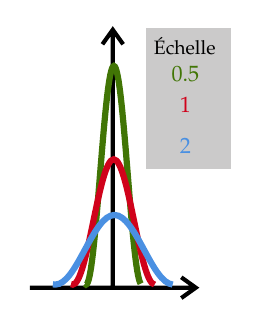
\begin{tikzpicture}[x=0.75pt,y=0.75pt,yscale=-1,xscale=1]
%uncomment if require: \path (0,300); %set diagram left start at 0, and has height of 300

%Shape: Axis 2D [id:dp18693685040272978] 
\draw [line width=1.5]  (119.83,151.67) -- (199.83,151.67)(159.83,27.4) -- (159.83,151.67) (192.83,146.67) -- (199.83,151.67) -- (192.83,156.67) (154.83,34.4) -- (159.83,27.4) -- (164.83,34.4)  ;
%Shape: Wave [id:dp5641937191696826] 
\draw  [color={rgb, 255:red, 65; green, 117; blue, 5 }  ,draw opacity=1 ][line width=2.25]  (146.41,149.77) .. controls (146.59,150.04) and (146.77,150.18) .. (146.95,150.18) .. controls (149.38,150.18) and (151.47,124.5) .. (153.66,97.51) .. controls (155.85,70.53) and (157.94,44.84) .. (160.37,44.84) .. controls (162.8,44.84) and (164.89,70.53) .. (167.08,97.51) .. controls (169.1,122.49) and (171.05,146.35) .. (173.25,149.77) ;
%Shape: Wave [id:dp9736357574926828] 
\draw  [color={rgb, 255:red, 208; green, 2; blue, 27 }  ,draw opacity=1 ][line width=2.25]  (139.7,149.94) .. controls (139.97,150.1) and (140.23,150.18) .. (140.5,150.18) .. controls (144.08,150.18) and (147.17,135.46) .. (150.39,119.99) .. controls (153.62,104.52) and (156.71,89.8) .. (160.29,89.8) .. controls (163.87,89.8) and (166.96,104.52) .. (170.19,119.99) .. controls (173.38,135.28) and (176.43,149.85) .. (179.96,150.18) ;
%Shape: Wave [id:dp9806953027168039] 
\draw  [color={rgb, 255:red, 74; green, 144; blue, 226 }  ,draw opacity=1 ][line width=2.25]  (130.98,150.05) .. controls (131.36,150.14) and (131.74,150.18) .. (132.12,150.18) .. controls (137.28,150.18) and (141.73,142) .. (146.38,133.41) .. controls (151.03,124.82) and (155.48,116.64) .. (160.64,116.64) .. controls (165.8,116.64) and (170.25,124.82) .. (174.9,133.41) .. controls (179.4,141.74) and (183.72,149.68) .. (188.68,150.16) ;
%Shape: Rectangle [id:dp4682062525043522] 
\draw  [draw opacity=0][fill={rgb, 255:red, 203; green, 202; blue, 202 }  ,fill opacity=1 ] (176,26.67) -- (216.83,26.67) -- (216.83,94.67) -- (176,94.67) -- cycle ;

% Text Node
\draw (178.42,29.67) node [anchor=north west][inner sep=0.75pt]  [font=\scriptsize,color={rgb, 255:red, 0; green, 0; blue, 0 }  ,opacity=1 ] [align=left] {Échelle};
% Text Node
\draw (186.92,43.67) node [anchor=north west][inner sep=0.75pt]  [font=\footnotesize,color={rgb, 255:red, 65; green, 117; blue, 5 }  ,opacity=1 ] [align=left] {0.5};
% Text Node
\draw (190.92,58.67) node [anchor=north west][inner sep=0.75pt]  [font=\footnotesize,color={rgb, 255:red, 208; green, 2; blue, 27 }  ,opacity=1 ] [align=left] {1};
% Text Node
\draw (190.92,78.67) node [anchor=north west][inner sep=0.75pt]  [font=\footnotesize,color={rgb, 255:red, 74; green, 144; blue, 226 }  ,opacity=1 ] [align=left] {2};


\end{tikzpicture}
		\end{center}
	\item[de fréquence]	L'interprétation dépend du contexte.
		\begin{itemize}
		\item	\og \textit{rate parameter} \fg{};
		\item	Dans le cas d'un processus de Poisson, le paramètre de fréquence décrit le taux auquel les événements se produisent;
		\item	Souvent, il est défini comme le réciproque du paramètre d'échelle pour indiquer le taux de déclin d'une fonction exponentielle;
		\item	Des valeurs près de 1 impliquent un déclin lent alors que des valeurs près de 0 impliquent un déclin rapide.
		\end{itemize}
%%%		https://www.statisticshowto.com/location-parameter/
	\item[d'emplacement]	Stipule où la densité est située.
		\begin{itemize}
		\item	\og \textit{location parameter} \fg{};
		\item	Plus précisément, indique où sur l'axe des $x$ la distribution est centrée relatif à la distribution normale standard;
		\item	Une distribution normale standard est centrée à 0 donc un paramètre d'emplacement de 5 implique que la densité est centrée à $x	=	5$.
		\end{itemize}
\end{description}


\begin{distributions}[Notation]
\begin{description}
	\item[$S$]	Les coûts d'un portefeuille.
	\item[$\rho(S)$]	Une mesure de risque.
\end{description}
\end{distributions}



\pagebreak

\section{Preuves}

\subsection*{\hypertarget{proof:ftc-quantile}{Preuve du théorème de la fonction quantile}}
\begin{formula}{}
\begin{align*}
	F_{F_{X}^{-1}(U)}
	&=	\Pr\left(F_{X}^{-1}(U) \leq x\right)	\\
	&\overset{2}{=}	\Pr\left(U \leq F_{X}(x)\right)	\\
	&\overset{1}{=}	F_{X}(x)
\end{align*}
\begin{enumerate}
	\item	Pour $U \sim Unif(0, 1)$, $F_{U}(u)	=	\Pr(U	\leq	u)	=	u$ alors $F_{U}(F_{X}(x))	=	F_{X}(x)$.
	\item	On doit prouver que:
		\begin{align*}
		\bigg\{	F_{X}^{-1}(U)	\leq	x	\bigg\}
		\equiv
		\bigg\{	U	\leq	F_{X}(x)	\bigg\}
		\end{align*}
\end{enumerate}

\tcbline

\paragraph{Cas 1:	$X$ est une variable aléatoire continue}
\begin{itemize}
	\item	Alors, l'équivalence est vraie puisque $\{	F_{X}^{-1}(U)	\leq	x	\}$ est la solution unique à $\{	U	\leq	F_{X}(x)	\}$ par définition.
\end{itemize}

\paragraph{Cas 2:	$X$ est une variable aléatoire quelconque}
\begin{enumerate}
	\item	On fixe \lfbox[conditions]{$x	=	F_{X}^{-1}(u)	=	\inf\{y \in \mathbb{R}; F_{X}(y)	\geq u\}$} ;
		\begin{itemize}
		\item	Donc, ce "$x$" est une valeur parmi les valeurs "$y$" qui rencontre la condition $F_{X}(y)	\geq	u$ ;
		\item	Il s'ensuit que puisque $u \leq F_{X}(y)$ alors \lfbox[conditions]{$u \leq F_{X}(x)$}.
		\end{itemize}
		\begin{align*}
		\bigg\{	F_{X}^{-1}(U)	\leq	x	\bigg\}
		\Rightarrow
		\bigg\{	U	\leq	F_{X}(x)	\bigg\}
		\end{align*}
	\item	On fixe \lfbox[conditions]{$u \leq F_{X}(x)$} ;
		\begin{itemize}
		\item	Puisque la fonction quantile est la plus petite valeur de $y$ tel que $u \leq F_{X}(y)$, il s'ensuit que $F_{X}^{-1}(u)	\leq  x$.
		\end{itemize}
		\begin{align*}
		\bigg\{	U	\leq	F_{X}(x)	\bigg\}
		\Rightarrow
		\bigg\{	F_{X}^{-1}(U)	\leq	x	\bigg\}
		\end{align*}
\end{enumerate}
Donc :
\begin{align*}
	\bigg\{	F_{X}^{-1}(U)	\leq	x	\bigg\}
	\equiv
	\bigg\{	U	\leq	F_{X}(x)	\bigg\}
\end{align*}
\end{formula}



\end{multicols*}
\end{document}


